%%---------------------------------------------------------------------------%%
%% refactor_planning.tex
%% Mike Buksas
%% $Id$
%%---------------------------------------------------------------------------%%
\documentclass[memo]{ResearchNote}
\usepackage[centertags]{amsmath}
\usepackage{amssymb,amsthm,graphicx}
\usepackage[mathcal]{euscript}
\usepackage{tmadd,tmath}
\usepackage{cite}

%%---------------------------------------------------------------------------%%
%% DEFINE SPECIFIC ENVIRONMENTS HERE
%%---------------------------------------------------------------------------%%
%\newcommand{\elfit}{\ensuremath{\operatorname{Im}(-1/\epsilon(\vq,\omega)}}
%\msection{}-->section commands
%\tradem{}  -->add TM subscript to entry
%\ucatm{}   -->add trademark footnote about entry

%%---------------------------------------------------------------------------%%
%% BEGIN DOCUMENT
%%---------------------------------------------------------------------------%%
\begin{document}

%%---------------------------------------------------------------------------%%
%% OPTIONS FOR NOTE
%%---------------------------------------------------------------------------%%

\toms{Distribution}
%\toms{Joe Sixpak/XTM, MS B226}
\refno{CCS-4-}
\subject{Template}

%-------NO CHANGES
\divisionname{Computer and Computational Sciences Division}
\groupname{CCS-4:Transport Methods Group}
\fromms{Mike Buksas/CCS-4 D409}
\phone{(505)665--3677}
\originator{tme}
\typist{tme}
\date{\today}
%-------NO CHANGES

%-------OPTIONS
%\reference{NPB Star Reimbursable Project}
%\thru{P. D. Soran, XTM, MS B226}
%\enc{list}      
%\attachments{list}
%\cy{list}
%\encas
%\attachmentas
%\attachmentsas 
%-------OPTIONS

%%---------------------------------------------------------------------------%%
%% DISTRIBUTION LIST
%%---------------------------------------------------------------------------%%

\distribution {}

%%---------------------------------------------------------------------------%%
%% BEGIN NOTE
%%---------------------------------------------------------------------------%%

\opening

\section{Background on the Particle-transport refactor}

Particles are currently represented in a heirachy of classes. {\tt
  Particle}, the abstract base class, and two derived classes {\tt
  Grey\_particle} and {\tt Multigroup\_particle}. The interface of the
derived classes is a mixture of virtual and non-virtual functions.
Most classes which use particles are templated on the particle type
and do {\em not} refer to the particle via its base class. The purpose
of the base class is to provide a common set of inherited data and
methods (via protected code blocks) to the derived classes. The
principal difference between the two derived classes is the different
object used to contain opacity data and the different interface used
to access opacity data from the object.

The particle classes currently implement the main particle-transport
algorithm.  This algorithm is characterized by repeatedly computing
distances to various events which limit the streaming of particles.
Determining the shortest of these distances. Streaming the particle
that distance and tallying the results. Depending on the nature of the
event the particle can either live to be streamed again, perhaps
after accquiring a new direction (after scattering), or die and be
eliminated from the computation (e.g. absorption)

The addition of multigroup versus grey bifurcated this function into
versions for the grey and multigroup. These functions are {\em nearly
  identical}. They differ only in the handful of lines which are
concerned with the interface to the opacity object and processing
random walk events.

The addition of random walk to the transport process caused another
bifurcation in the transport functions, resulting in four functions
total. Each particle's transport split into versions suitable for
transport with random walk enabled, or not. These functions are also
nearly identical, differing only in the conditional logic for random
walks.

\section{The contractor model for particle transport}

The transport algorithm for a particle consists of repeated short
streaming steps which are limited by various events. These events then
cause a change in the state of the particle. The streaming steps are
repeated until the particle enters a state for which the streaming
stops. The particle can be dead, go to census, or need to be
communicated to another domain.

The contractor methaphor for particle transport differs from the
current approach in two main ways: First, it seperates the different
events which effect the transport process. Second, the contractor
metaphor changes the particle transport algorithm from something
implemented {\em by} the particle to somthing applied {\em to} the
particle. This change will enable different generic programming
techniques to unify the code.

Currently, the limiting events in the particle transport algorithm
are: collisions (which consists of absorption, effective scattering
and Thompson scattering), mesh boundary corssings, attaining weight
cutoff, and going into census. Optionally, particles can also undergo
random walk. Random walk is different in that it is not a
streaming-limiter but rather circumvents the streaming step.

Each of these events (or group of related sub-events e.g. collisions)
has two aspects to it: It generates a distance at which the event
occurs, and, if the event comes to pass, changes the state of the
particle to reflect the event. This change in state can include
resampling its direction (for collisions) resampling its position
(for random walk), killing the particle, moving it to census,
etc. Both of these steps generally require the collaboration of other
objects which hold needed data. For example, the mesh to determine the
distance to boundary crossings, or the opacity to determine the
distance to cutoff.

In the contractor model, the more complicated limiting events would be
implemented as seperate classes. This class computes the event
distance and modifies the particle state as seperate methods. These
methods take the particle in question as arguments. Less complicated
limiting events may not require offloading into seperate classes, but
should still be expresses as pairs of functions in the same pattern.

With the limiting event compuations and implementations moved into
seperate classes or functions, the main loop of the particle transport
algorithm contains less data and is less complicated. It is primairly
responsible for soliciting distance information from its various
contractors, (e.g. ``bids''), determining which event occurs (the
``winner'') and handing the particle to that contractor for
implementation.

\section{Contractor implemetation details by example}

A good candidate for stand-alone contractor status is the collision
event handler. This event depends on additional data extracted from
the opacity class and computes probabilities from this data. Also,
its effect of the particle involves conditionals on the particle's
state (analog versus implicit absorption). This is a fair amount of
complexity which should be encapsulated. This will also isolate the
main particle-transport algorithm from the details in the event that
they should change. We take a closer look at this contractor as an
example here. An example implementation is illustrated in
Figure~\ref{fig:collision_contractor}

\begin{center}
  \begin{figure}
    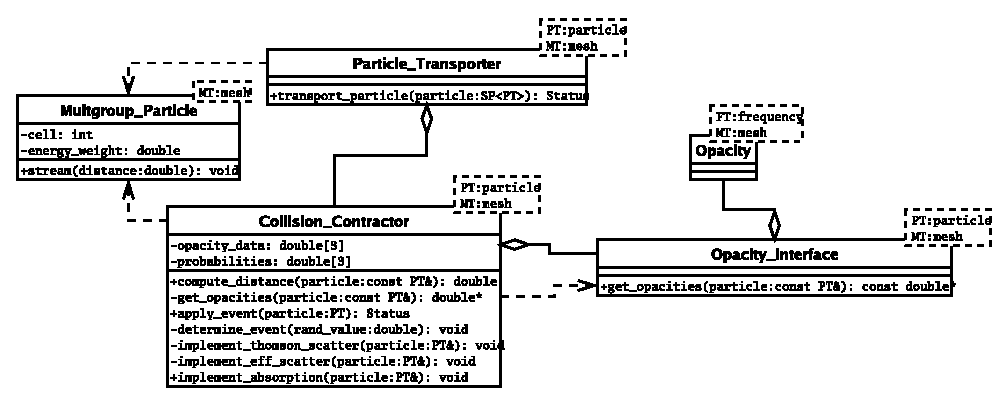
\includegraphics[width=6.5in]{figures/collision_contractor.eps}
    \caption{Example contractor implementation (not all members shown)} 
    \label{fig:collision_contractor}
  \end{figure}
\end{center}

Publicly, the  {\tt  Collision\_Contractor}  class will implement  {\tt
  compute\_distance} and  {\tt apply\_event} members.  The function {\tt
  compute\_distance} can take    a constant reference to  the  particle
while {\tt apply\_event} will need an ordinary  reference to modify the
particle.  Internally,  it will use  the opacity object to compute the
distance and the  relative probabilities for  its various sub-events. 
If it wins, the {\tt apply\_event} member function will dispatch to
vartious private members depending on the sub-event.

One of the problems that needs to be addressed when unifying the
manifold particle transport implementations is the differing interface
between the {\tt Opacity} class for grey frequency and multigroup
transport. The multigroup version contains an extra argument for the
energy group of the particle. We propose to wrap the opacity class
with another class which takes the particle as an argument and returns
the correct opacity information for its cell and group (if
applicable)

This wrapper class will be specialized on the frequency type (which is
part of the type of the particle class). The specialized versions will
differ in the following ways: They will contain the correct type of
opacity object, extract different data from the particle object (cell
and group versus just cell) and fetch the opacity information from the
opacity object via the correct interface).

This wrapper class will then in turn be used by the collision event
contractor in the particle transport algorithm. This class will also
need to be templated on the frequency type of the particle. This, in
turn, implys that the particle transporter class itself needs to be
templated on this parameter.

In various classes we can choose between templating on the particle
type itself or just the frequency type. In making the transition
between the two, we need to be able to extract the frequency type from
the particle type, or build the particle type from the frequecny type
(by combining it with other type information, e.g. mesh type). We give
one likely assignment of template parameters in
Figure~\ref{fig:collision_contractor}. In this implementation, class
{\tt Opacity\_Interface} extracts the frequency type partameter {\tt
  FT} from the particle type {\tt PT} to determine the correct
parameter for the {\tt Opacity} class. 

\section{Implementation of random-walk and particle-transport algorithm}

With contractor classes (or functions) in place for the limiting
events, we reduce the main particle transport algorithm to the
following:

\begin{itemize}
  \item Accept a new particle for transporting
  \item Do new-particle initializations (e.g. initialize surface
    particle tracking)
  \item While the particle is ``alive'':
    \begin{enumerate}
    \item Obtain limiting distances from contractors
    \item Choose limiting event
    \item Pass particle to winning contractor.
    \item Post-process the streaming step (e.g. surface tracking)
    \end{enumerate}
  \item Post-process transport step. E.g. tally fate of particle.
\end{itemize}

Most of the complication lies in step 2. Most of this is the result of
random walk. Among the streaming-distance limiters, the winner is
always the one with the shortest distance. Random walk is preferred
over collisions if its distance is greater, but its distance must be
less than the distance to census. 

Other complications involving random walk is that it may not always
be enabled and must be disabled in cells in which a tally surface is
present. Random walk is also only possible if the particle is in
certain states. The effect of random walk on a particle also differ
with the frequency type. Finally, random walk can send a particle
straight to census. 

Some of these complications can be moved into the random walk
implementation either by adding to the existing class or wrapping it
in a contractor-style interface class. Wrapping the random walk in
another class would provide a better location for the
frequency-specific specializations. The interactions between random
walk and other limiting events should be handled in the particle
transport algorithm.

Currently, the random walk option is checked for only once before
dispatching to the different transport functions in the particle.
Unifying these functions will require a conditional check on random
walk with each streaming step. This carries a performance penalty that
we will address later.

\section{Proposed sequence for refactoring}

Our first objective for this sub-project is to unify the four
implementations of the particle transport alforithm. On outline of our
proposed approach to do so are as follows:

\begin{itemize}
\item Unify the logic between the random-walk and non-random walk
  transport versions. 

  \begin{itemize} 
  \item Group the detection and execution of random walk
    together. 
  \item Wrap the random walk detection/execution in a conditional
    (This can be done via conditionals on the {\tt Random\_Walk} smart
    pointer.
  \item At this point, it should be possible to combine the two
    functions.
  \end{itemize}

\item Create Particle-transporter class. This class will take over the
  transport operation.

  \begin{itemize}
  \item Template the class on the Particle type: Grey (G) or
    Multigroup (MG). This can be done with a flag class or the full
    type of the particle.
  \item Create specialized versions of the transport algorithm in the
    particle-transporter.
  \item Expand the public interface of the Particle classes, if
    necessary, to enable the transport methods in the
    particle-transporter to function. Various other methods of the
    Particle class can also be moved over to the transporter as
    needed.
  \item Construct the particle-transporter with references or pointers
    to classes which provide information for doing the transport:
    e.g. opacity, mesh.
  \end{itemize}

\item Unify the Grey and Multigroup specializations in the particle
  transporter by creating a collision event contractor class. 

  The collison handler will compute distance to collisions and
  implement the streaming operation when a stream-to collision
  takes place. 

  \begin{itemize}
    \item Create class and template on particle type.
    \item Implement distance computation (``bidding'') and streaming
      operator (``winning''). These functions take a particle
      argument.
    \item Construct with needed assistant classes. e.g. opacity.
    \item Modify the particle transporter to use the collision event
      contractor.
    \item The Grey and Multigroup specializations of the transport
      function should now differ only in types, so we can eliminate
      the specializations.
    \end{itemize}
    
  \item Evaluate the use of contractors to handle remaining events:
    Mesh crossing, Census, Termination, Random Walk. The process would
    be similar to that for the Collision Constractor.
    
  \item Remove the old transport methods in particle classes. Remove
    unnecessary data types and data objects.
    
  \item Modify client codes to create and use a particle-transporter
    class instead of calling the particle-transport method.

\end{itemize}

\section{Next Steps}

Some other changes to the code may follow logically after the
refactoring above. We list some of those here.

\begin{itemize}
\item Eliminate mesh dependency from Particle.

  Since the particle will no longer logically depend on the mesh, the
  mesh type template parameter can probably be removed from the
  particle type. 
      
\item Collapse particle hierarchy. 
  
  Since most of the differing code will have been removed, the
  particle hierarchy is ripe for being collapsed into a single class.
  The new particle class would be templated on the frequency type and
  use a ``mixin'' style component to add the extra members needed by
  the multigroup type.

\item Eliminate cutoff as a limiting event.

  Weight-based cutoff can be changed from a limiting event to a stream
  post-processing event. This will speed up transport, since the
  distance to cutoff computation is logarithmic. It will also simplify
  the particle-transport loop somewhat.

  It will, however, change the regression test results.

\item Statically bind random-walk
  
  We can look for a way to use template parameters to statically build
  versions of the particle-transport algorithm with and without random
  walk. Since these particle transporters will have different types,
  the algorithm would be called via and interface in an abstract base
  class. Since the virtual function call would only be at the
  beginning of the particle transport algorithm, the cost is likely
  negligible.
  
\item Statically bind surface-tracking. 

  As with random walk, we can use template parameter object to build
  two versions of the particle transport algorithm with and without
  surface tracking. Since surface tracking interacts with random walk,
  statically binding both may be impractically complicated. 

\end{itemize}
  
 
\closing
\end{document}

%%---------------------------------------------------------------------------%%
%% end of refactor_planning.tex
%%---------------------------------------------------------------------------%%
